
Za usporedbu, odabranu su sljedeća četiri modela:

\begin{itemize}
    \item R+TI baseline - arhitektura Riffusion\cite{{forsgren2022riffusion}} uz korištenje tekstualne inverzije (engl. \textit{Textual Inversion})\cite{gal2022imageworthwordpersonalizing} 
    \item SS VQ-VAE - varijacijski autoenkoder s vektoriziranom latentnom reprezentacijom učen samonadzirano, korišten za prijenos stila glazbe na temelju jednog primjera (engl. \textit{One-shot music style transfer}) \cite{Cifka_2021}
    \item MUSICGEN - jezični model za tekstom vođen prijenos stila glazbe uvjetovan melodijom (engl. \textit{Text-Guided Music Stylization with Melody Conditioning})\cite{copet2024simplecontrollablemusicgeneration}
    \item Originalni model iz reproduciranog rada\cite{huang2024musicstyletransferdiffusion}
\end{itemize}

\begin{table}[H]
    \centering
    \caption{Usporedba mjera dobrote različitih modela}
    \label{table:usporedne_mjere}
    \begin{tabular}{ |c|c|c| }
        \hline
        Model & CP& SF \\
        \hline
        R+TI\cite{forsgren2022riffusion}\cite{gal2022imageworthwordpersonalizing} & 0.35 & 0.27 \\
        SS VQ-VAE\cite{Cifka_2021} & 0.24 & 0.28 \\
        MUSICGEN\cite{copet2024simplecontrollablemusicgeneration} & 0.28 & 0.24 \\
        Originalni model\cite{huang2024musicstyletransferdiffusion} & \textbf{0.46} & 0.28 \\
        \hline
        Naš model & 0.41 & \textbf{0.43} \\
        \hline
    \end{tabular}
\end{table}

U tablici~\ref{table:usporedne_mjere} možemo vidjeti iznos mjera očuvanja sadržaja i podudaranja stila za različite modele. Važno je napomenuti da je u slučaju odabranih modela mjera podudaranja stila izračunata na temelju ugrađivanja stiliziranih zvučnih zapisa i tekstualnih opisa stila, dok su za naš model ugrađivanja tekstualnih opisa stila zamijenjeni prosječnim ugrađivanjem zvučnih zapisa stila. U slučaju našeg modela, prikazane su prosječne mjere dobrote preko sva tri odabrana stila.

Možemo vidjeti da originalni model koji reproduciramo\cite{huang2024musicstyletransferdiffusion}, kao i naš model, imaju bolji iznos obje mjere dobrote od preostalih odabranih modela za prijenos stila. Ako uspoređujemo našu implementaciju s originalnom, vidimo da originalni model ima nešto viši iznos mjere očuvanja sadržaja, dok naš model ima viši iznos podudaranja stila. Naravno, odnos očuvanja sadržaja i podudaranja stila veoma ovisi o konkretnom iznosu hiperparametara \textit{scale} i \textit{strength}. Veći iznos očuvanja sadržaja mogli bismo lako postići povećavanjem iznosa hiperparametra \textit{strength}, ali po cijenu nižeg podudaranja stila.

Osim izračuna mjera dobrote za cijeli skup zvučnih zapisa sadržaja, dodatno smo za svaki naučeni stil pronašli primjere koji imaju najveći iznos mjere očuvanja sadržaja odnosno mjere podudaranja stila. Na slici \ref{fig:cp_comp} možemo vidjeti jedan od mel-spektrograma stila korišten za učenje modela, originalni mel-spektrogram sadržaja i stilizirani mel-spektrogram sadržaja za koji je iznos mjere očuvanja sadržaja najveći. S druge strane, na slici \ref{fig:sf_comp} možemo vidjeti jedan od mel-spektrograma stila korišten za učenje modela, originalni mel-spektrogram sadržaja i stilizirani mel-spektrogram sadržaja za koji je iznos mjere podudaranja stila sadržaja najveći.

\begin{figure}
    \centering
    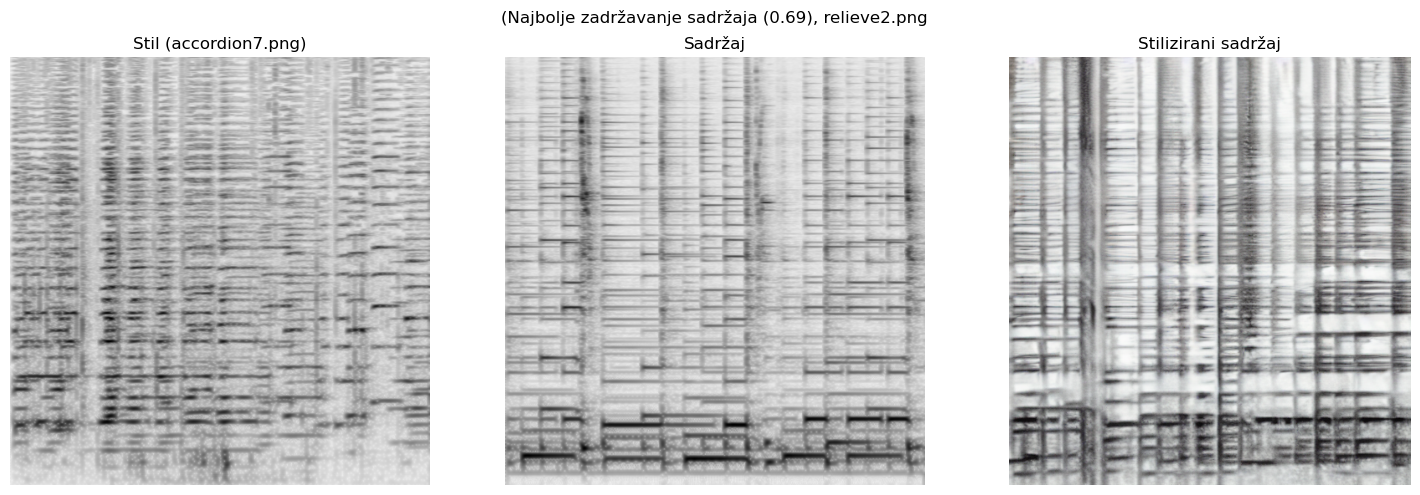
\includegraphics[width=0.75\linewidth]{imgs/najboljisadrzaj.png}
    \caption{Spektrogram stila, originalnog primjera i stiliziranog primjera s najvećim očuvanjem sadržaja}
    \label{fig:cp_comp}
\end{figure}


\begin{figure}[H]
    \centering
    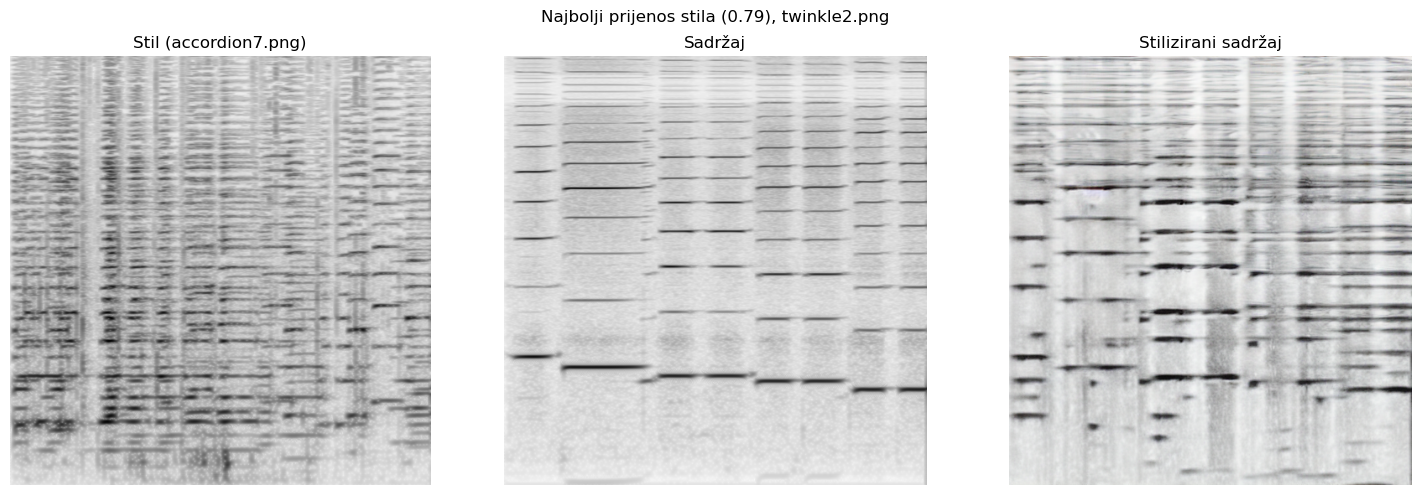
\includegraphics[width=0.75\linewidth]{imgs/najboljistil.png}
    \caption{Spektrogram stila, originalnog primjera i stiliziranog primjera s s najvećim prijenosom stila}
    \label{fig:sf_comp}
\end{figure}